%----------------------------------------------%
% Template Beamer para Apresentações da Asset1 %
%                 %
% Baseado em MIT Beamer Template			   %
% versao 1.1								   %
% Atualizado em 14/12/2021					   %
%----------------------------------------------%
% !TeX spellcheck = pt_BR
\documentclass[t,aspectratio=169]{beamer}
% Para alterar a linguagem do documento
\usepackage[portuges]{babel}
% Para aceitar caracteres especias deretamente do teclado
\usepackage[utf8]{inputenc}
% Para seguir as normas da ABNT de citacao e referencias
\usepackage[alf]{abntex2cite}
% Para incluir figuras
\usepackage{graphicx}
% Para melhor ajuste da posisao das figuras
\usepackage{float}
% Para ajustar as dimensoes do layout da pagina
\usepackage{geometry}
% Para formatar estrutura e informacoes de formulas matematicas
\usepackage{amsmath}
% Para incluir simbolos especiais em formulas matematicas
\usepackage{amssymb}
% Para incluir links nas referencias
\usepackage{url}
% Para incluir paginas de documentos .pdf externos
\usepackage{pgfpages}
% Para ajustar o estilo dos contadores
\usepackage{enumerate}
% Para modificar a cor do texto
\usepackage{color}
% Para incluir condicoes
\usepackage{ifthen}
% Para colocar legendas em algo que nao e float
\usepackage{capt-of}

\usepackage{hyperref}
\usepackage{fontspec}
\setmainfont[UprightFont={* Regular},BoldFont={* Bold},ItalicFont={* Medium}]{AmpleSoft Pro}

\let\sfdefault\rmdefault

% Para definir o tema do slide
\usetheme{Berlin}
% Para difinir cores e background
\usecolortheme{Asset1}
% Para numerar as figuras
\setbeamertemplate{caption}[numbered]
\beamertemplatenavigationsymbolsempty

% Título
\title[Comitê de Risco]{
	Comitê de Risco e Liquidez}

\titlegraphic{
	
\includegraphics[width=0.35\textwidth]{figuras/logo_Asset1}
}

% Data
\date{
	13-janeiro-2022}
% Autores
\author[\href{mailto:risco@asset1.com.br}{risco@asset1.com.br}]{
	\href{mailto:mauricio.pereira@asset1.com.br}{Maurício Pereira}\\
	\vspace{0.10cm}
	\href{mailto:luis.oliveira@asset1.com.br}{Luís Oliveira}
}
% Logo do canto inferior direito
\pgfdeclareimage[height=0.45cm]{logo_Asset1}{figuras/logo_Asset1}
\logo{
	\vspace*{-0.30cm}
	\pgfuseimage{logo_Asset1}
	\hspace*{-0.08cm}}


\begin{document}

%\frame{\titlepage}

{
	\setbeamertemplate{logo}{}
	\begin{frame}
		\maketitle
	\end{frame}
}

%%%%%%%%%%%%%%%%%%%%%%%%%%%%%%%%%%%%%%%%%%%%%%%%%%%%%%%%%%%%%
\section*{Agenda}
\begin{frame}{Agenda}
	\tableofcontents
\end{frame}

%%%%%%%%%%%%%%%%%%%%%%%%%%%%%%%%%%%%%%%%%%%%%%%%%%%%%%%%%%%%%
\section[Pendências]{Pontos Pendentes}
\begin{frame}{Pontos Pendentes}
	\begin{enumerate}
		\item Controle de Risco de Liquidez\\
		Em andamento
		%\item Modelagem de linha d'água\\
		%Concluído ({\color{green}\checkmark})
		\item Permissionamento do Banco de Dados\\
		Em andamento
	\end{enumerate}
\end{frame}

%%%%%%%%%%%%%%%%%%%%%%%%%%%%%%%%%%%%%%%%%%%%%%%%%%%%%%%%%%%%%
\section[Resultado]{Atribuição de Resultado}
\begin{frame}{Atribuição de Resultado por \emph{ESTRATÉGIA}}
	\centering
	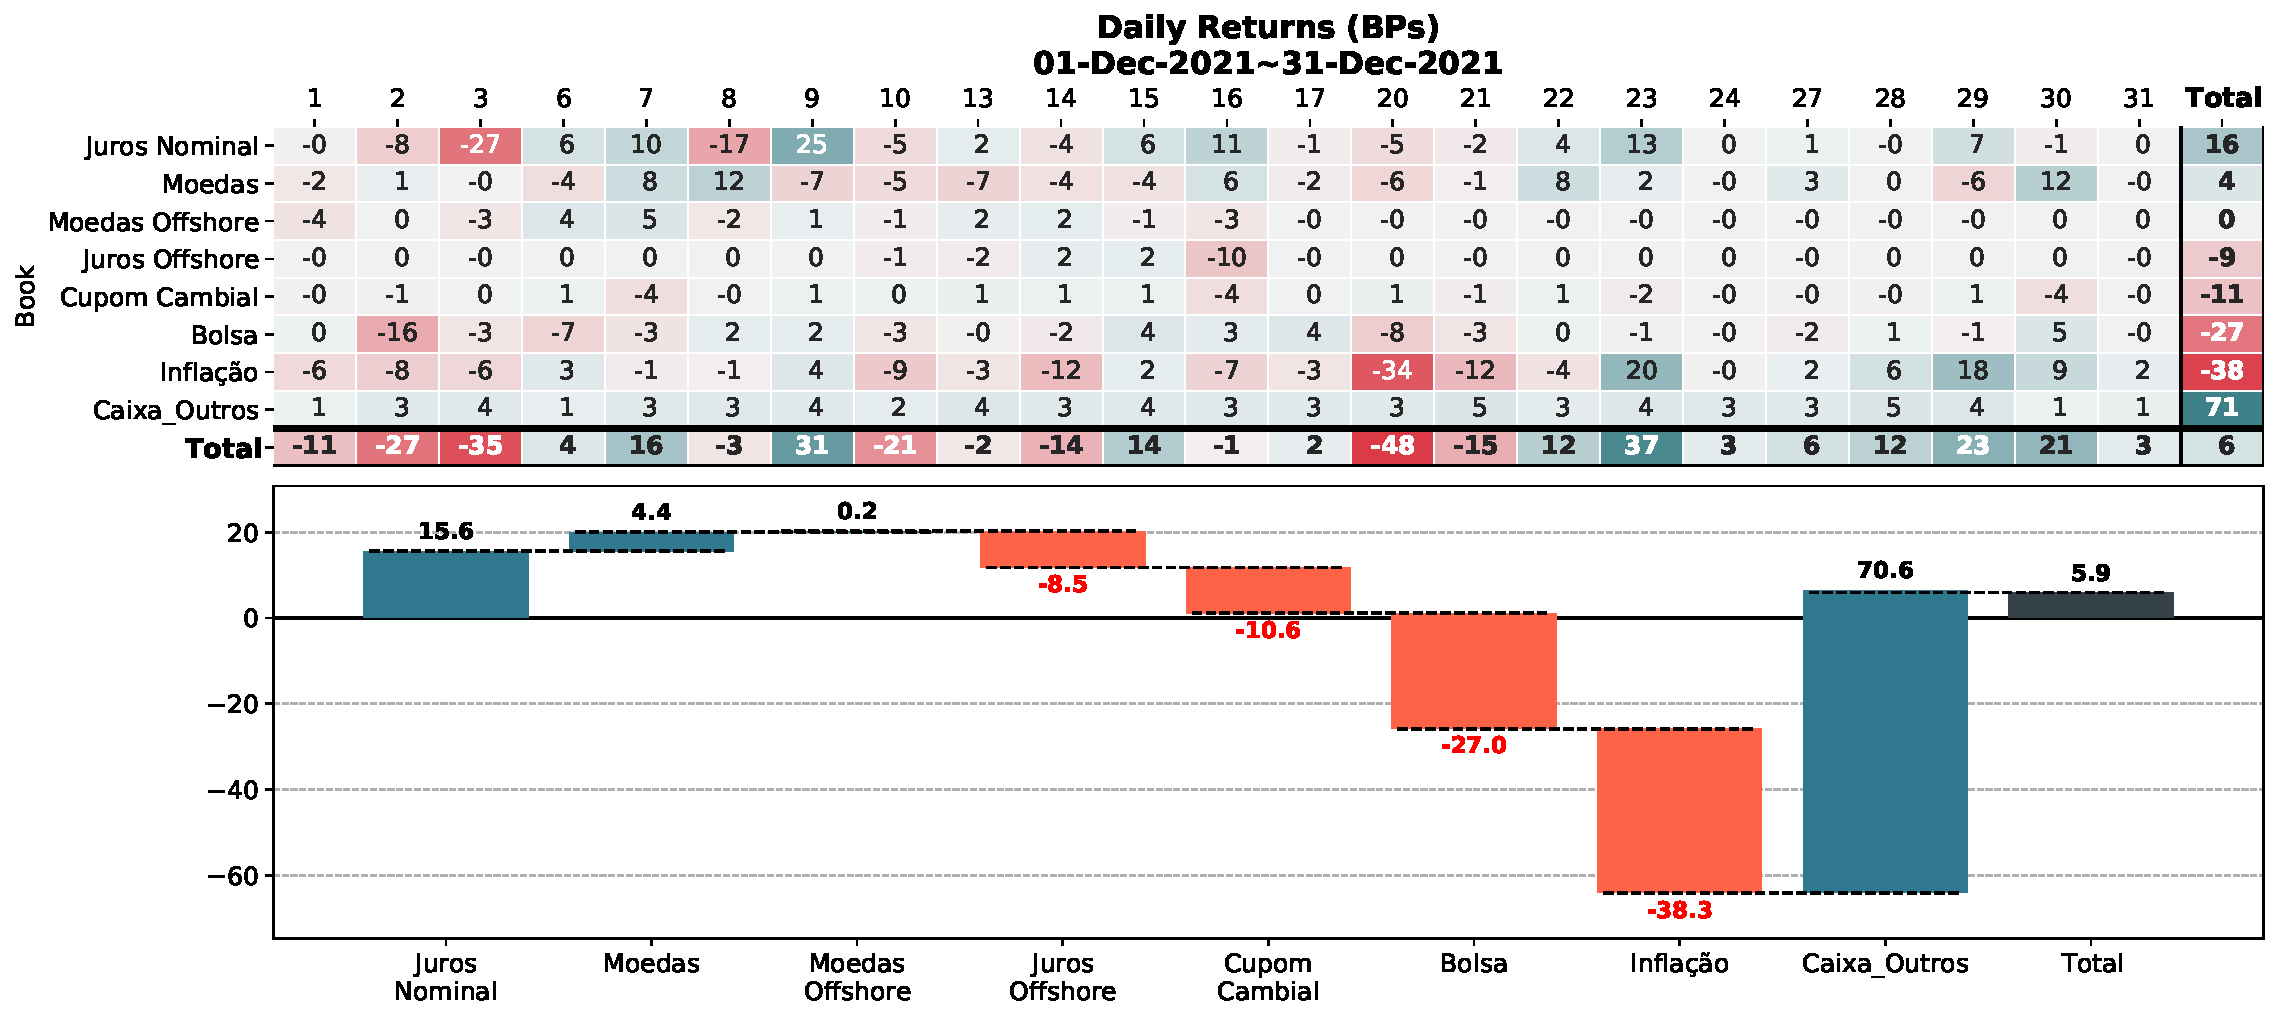
\includegraphics[width=0.99\textwidth]{figuras/211201_211231_pnl.pdf}%month_pnl.py
\end{frame}

\begin{frame}{Atribuição de Resultado por \emph{PRODUTO}}
	\centering
	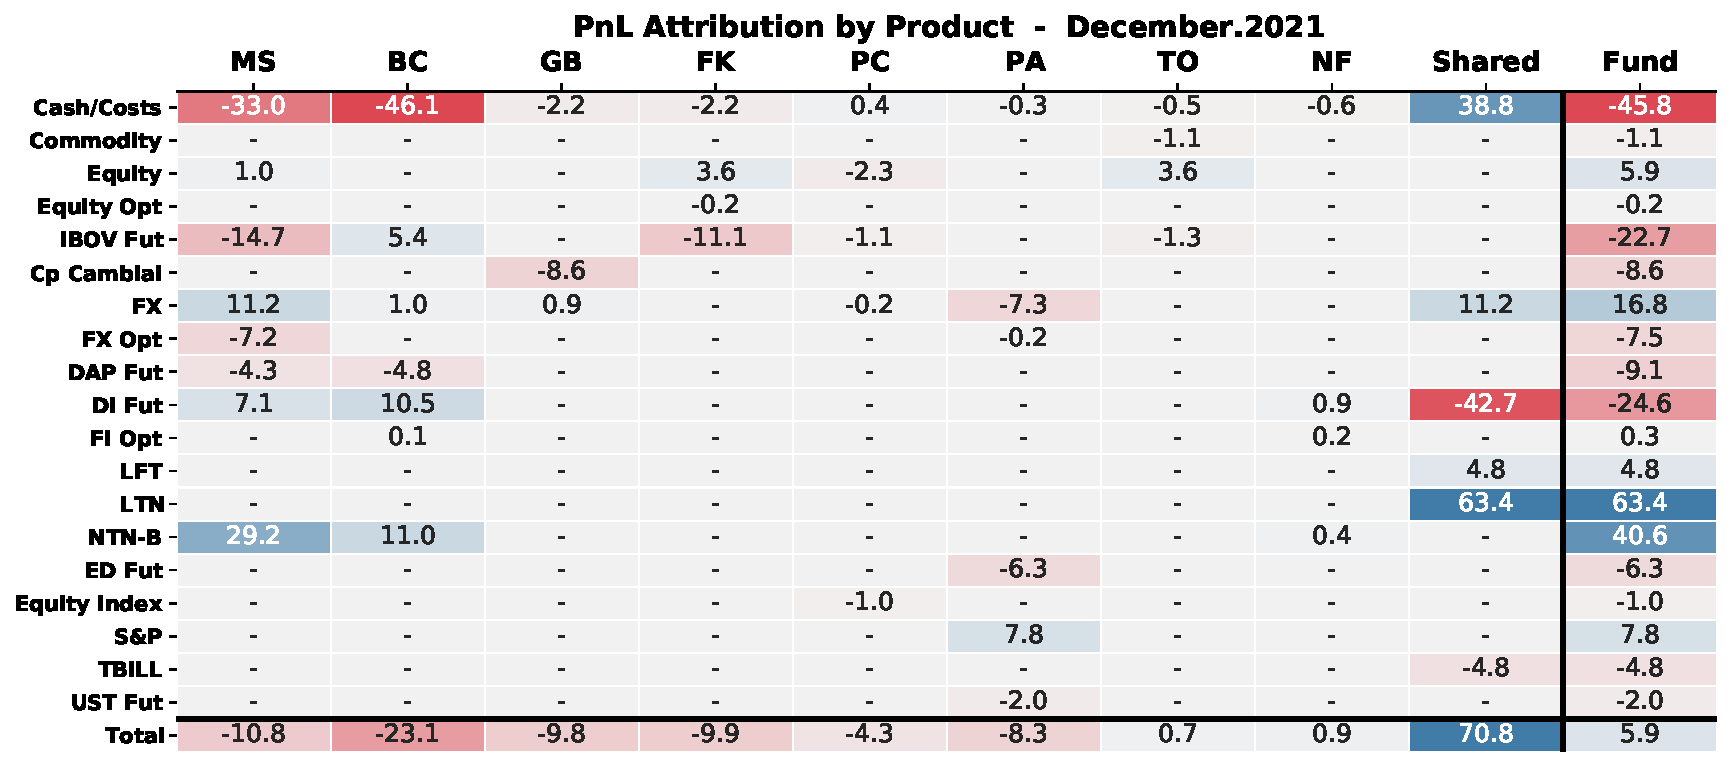
\includegraphics[width=0.99\textwidth]{figuras/20211231_A1 Master FIM_pnl_product.pdf}%pnl_perfattrib.py

\end{frame}

\begin{frame}{Performance Mensal}
	\centering
	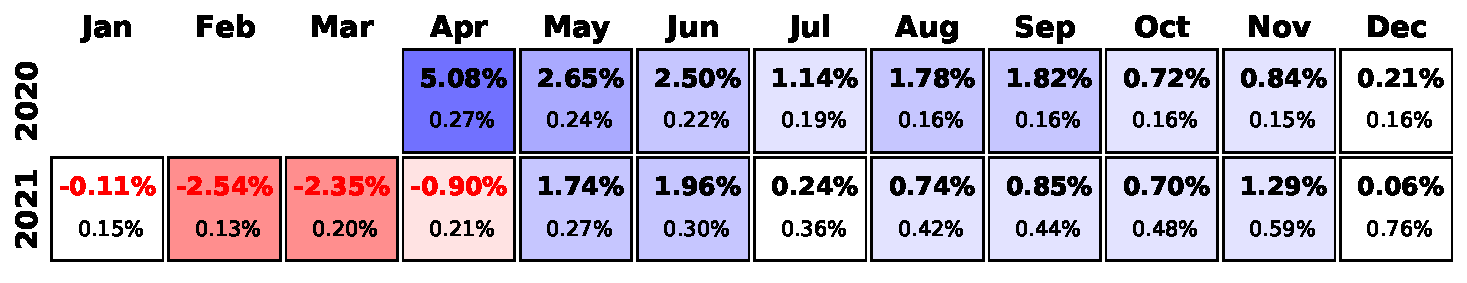
\includegraphics[width=0.99\textwidth]{figuras/20211231_A1 Master FIM_monthBymonth_performance.pdf} %risk_report/fund_performance.py
	\begin{itemize}
		\item \large{Retorno do Master (\%)}\\
		\small{Retorno do CDI (\%)}
	\end{itemize}
\end{frame}

\begin{frame}{Performance e Drawdown}
	\centering
	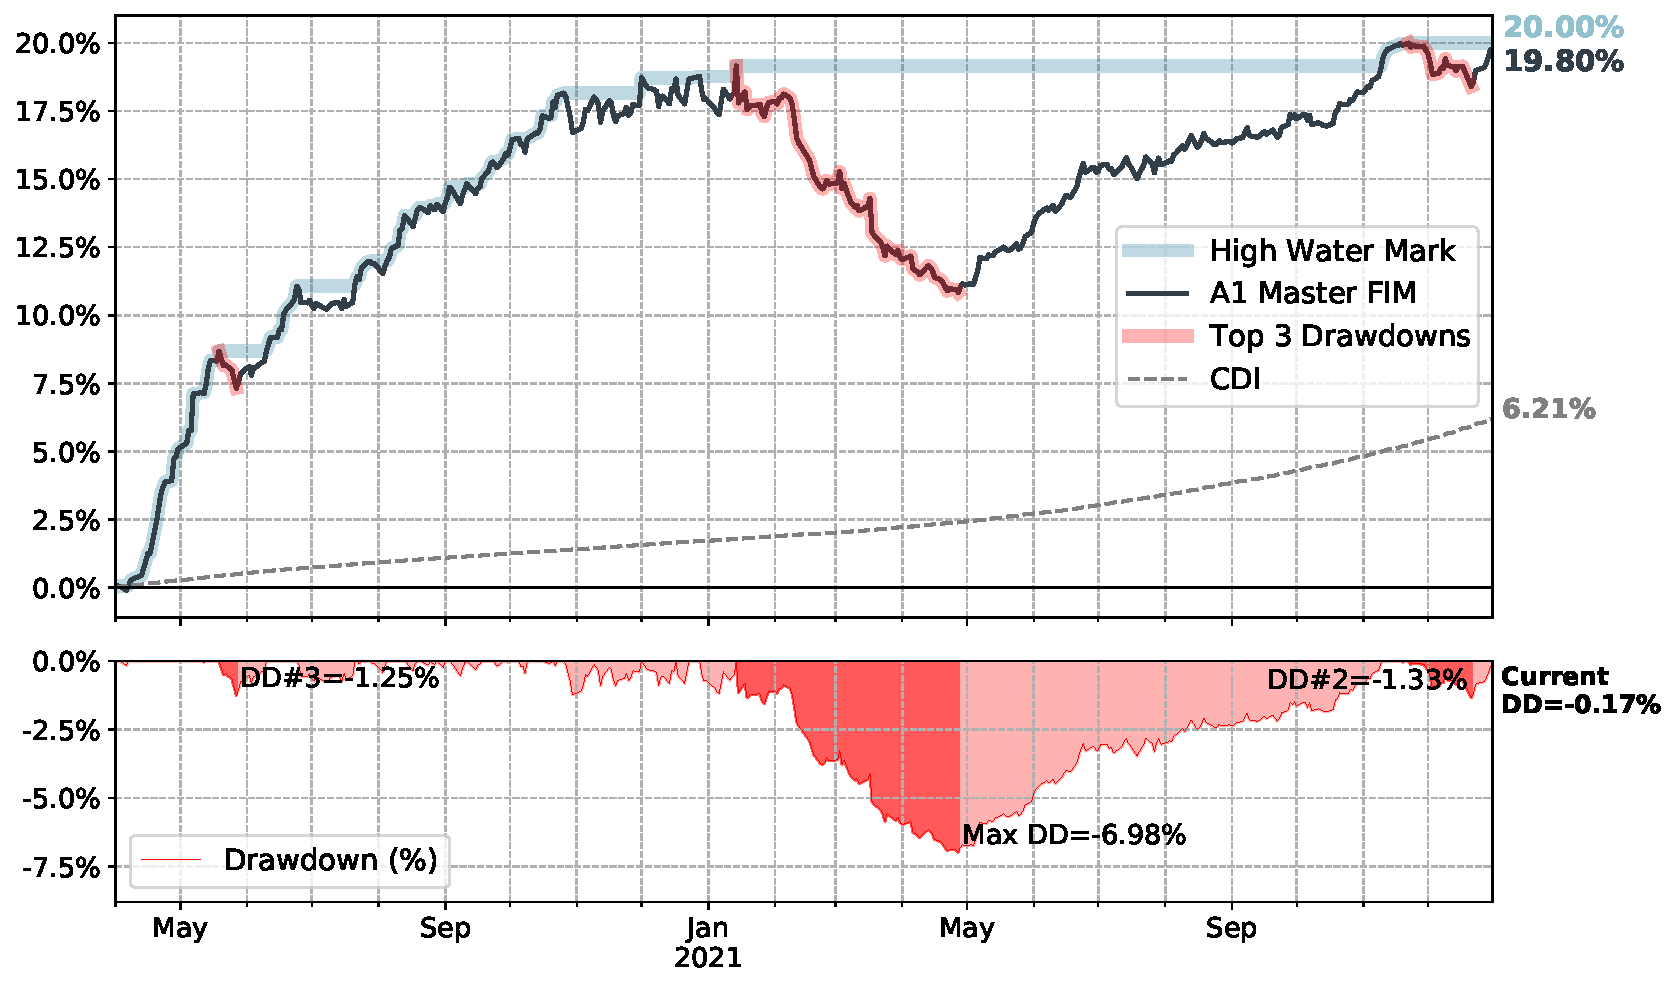
\includegraphics[width=0.75\textwidth]{figuras/20211231_A1 Master FIM_drawdown.pdf}  %risk_report/fund_drawdown.py
\end{frame}

%%%%%%%%%%%%%%%%%%%%%%%%%%%%%%%%%%%%%%%%%%%%%%%%%%%%%%%%%%%%%
\section[Carteira]{Revisão da Carteira}
\begin{frame}{Correlação entre estratégias}
	\centering
	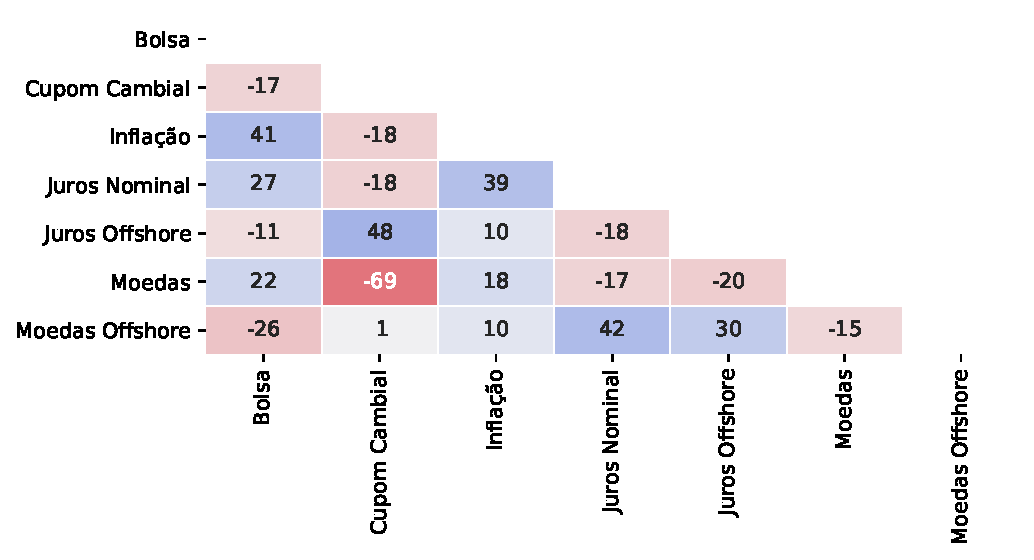
\includegraphics[width=0.85\textwidth]{figuras/211201_211231_correl.pdf} 
\end{frame}

\begin{frame}{V@R Backtest} 
	\begin{overlayarea}{\textwidth}{\textheight}
	\begin{columns}[T]
	\column[T]{0.30\linewidth}
	\begin{itemize}
		\item<1-> Houve \textbf{2} outliers no mês de {\color{blue1} dezembro}
			\begin{enumerate}
					\item<2->[2-dez]: VaR 23.5bps / PnL -27.3bps
					\item<3->[20-dez]: VaR 35.8bps / PnL -48.0bps
				\end{enumerate}
			
		\item<4-> Critério de Kupiec na zona de não-rejeição
		\item<5-> Critério de Christoffersen na zona de não-rejeição
	\end{itemize} 
	
	\column[T]{0.67\linewidth}
		\only<1>{
		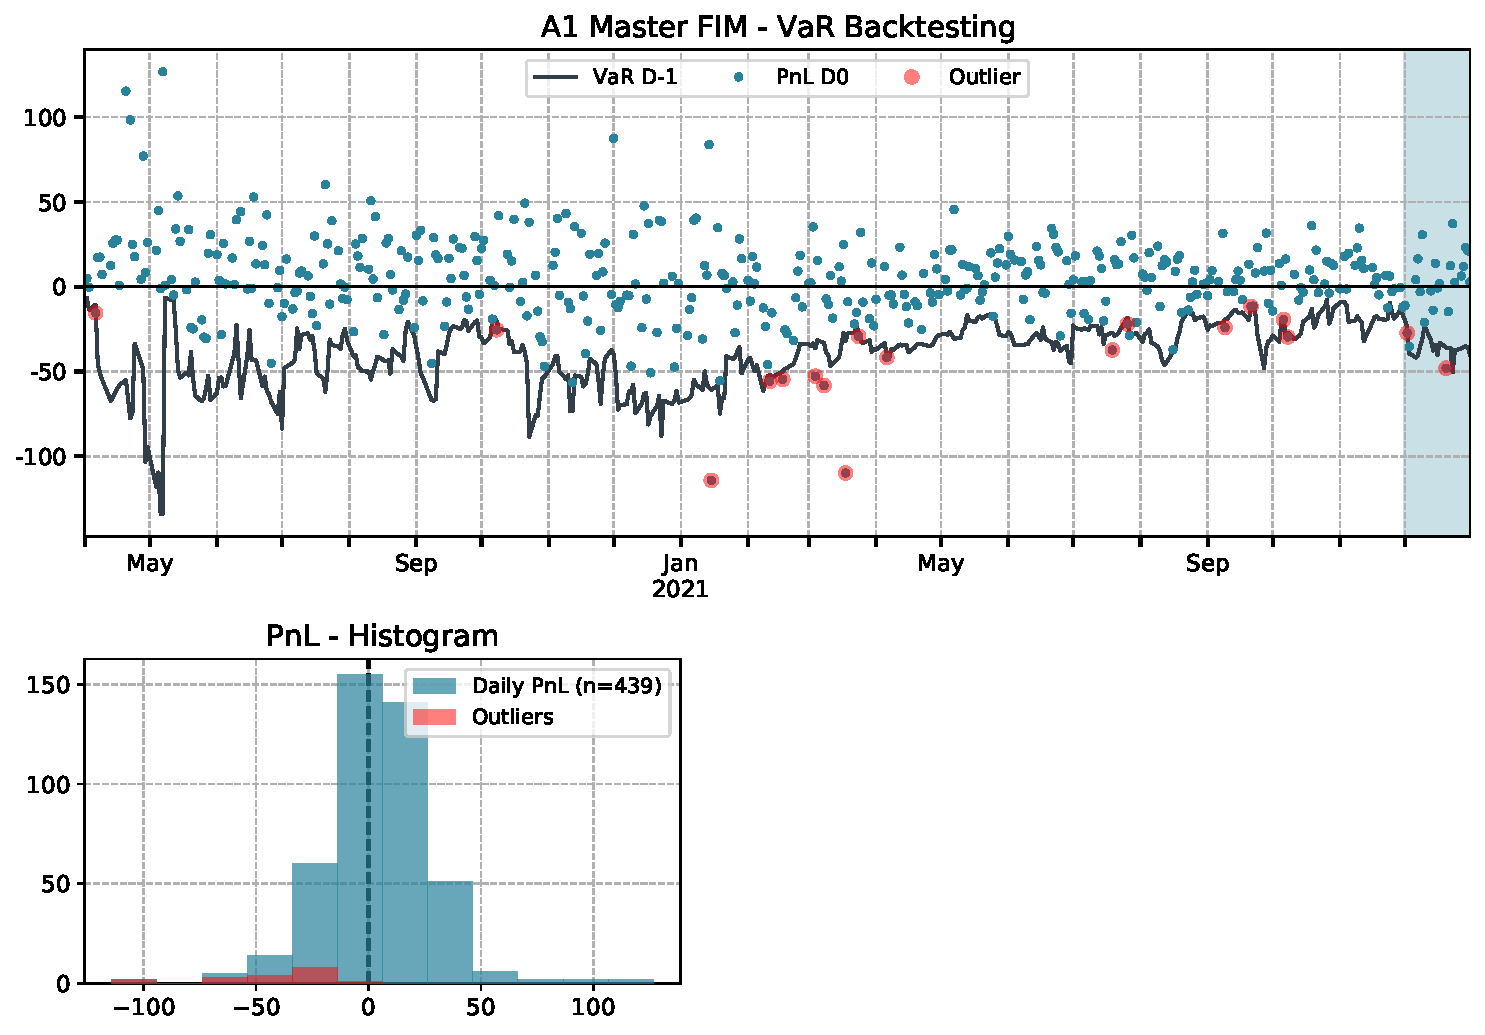
\includegraphics[width=0.90\linewidth]{figuras/20211231_A1 Master FIM_backtest_1.pdf}%backtest.py
		}	
		\only<2>{
		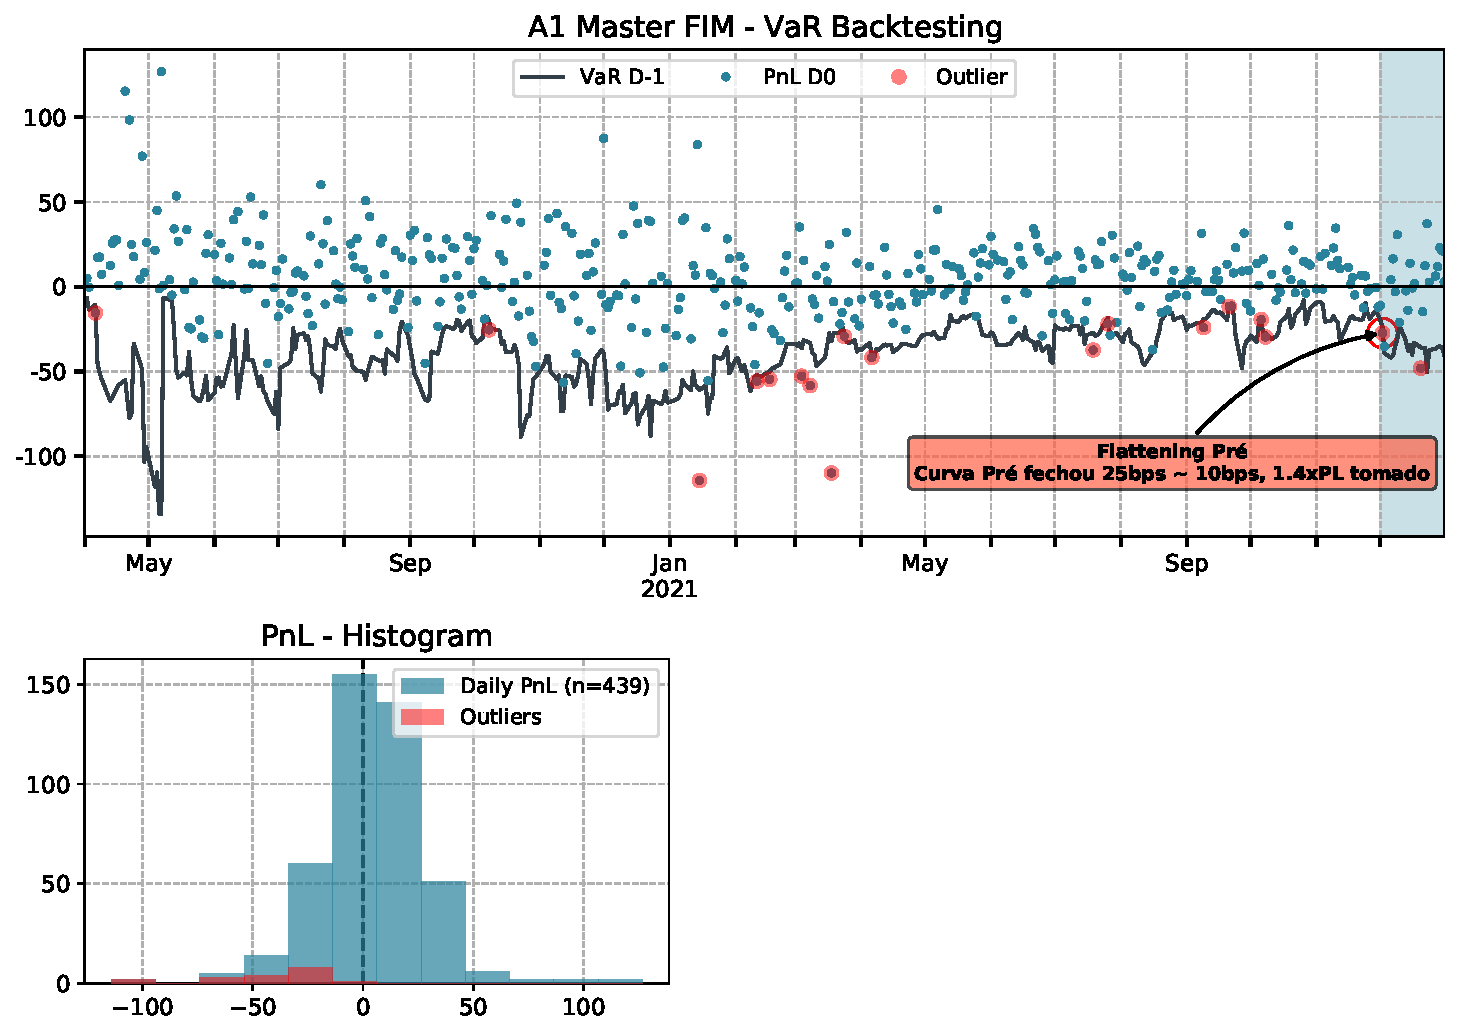
\includegraphics[width=0.90\linewidth]{figuras/20211231_A1 Master FIM_backtest_2021-12-02.pdf}
		}
		\only<3>{
			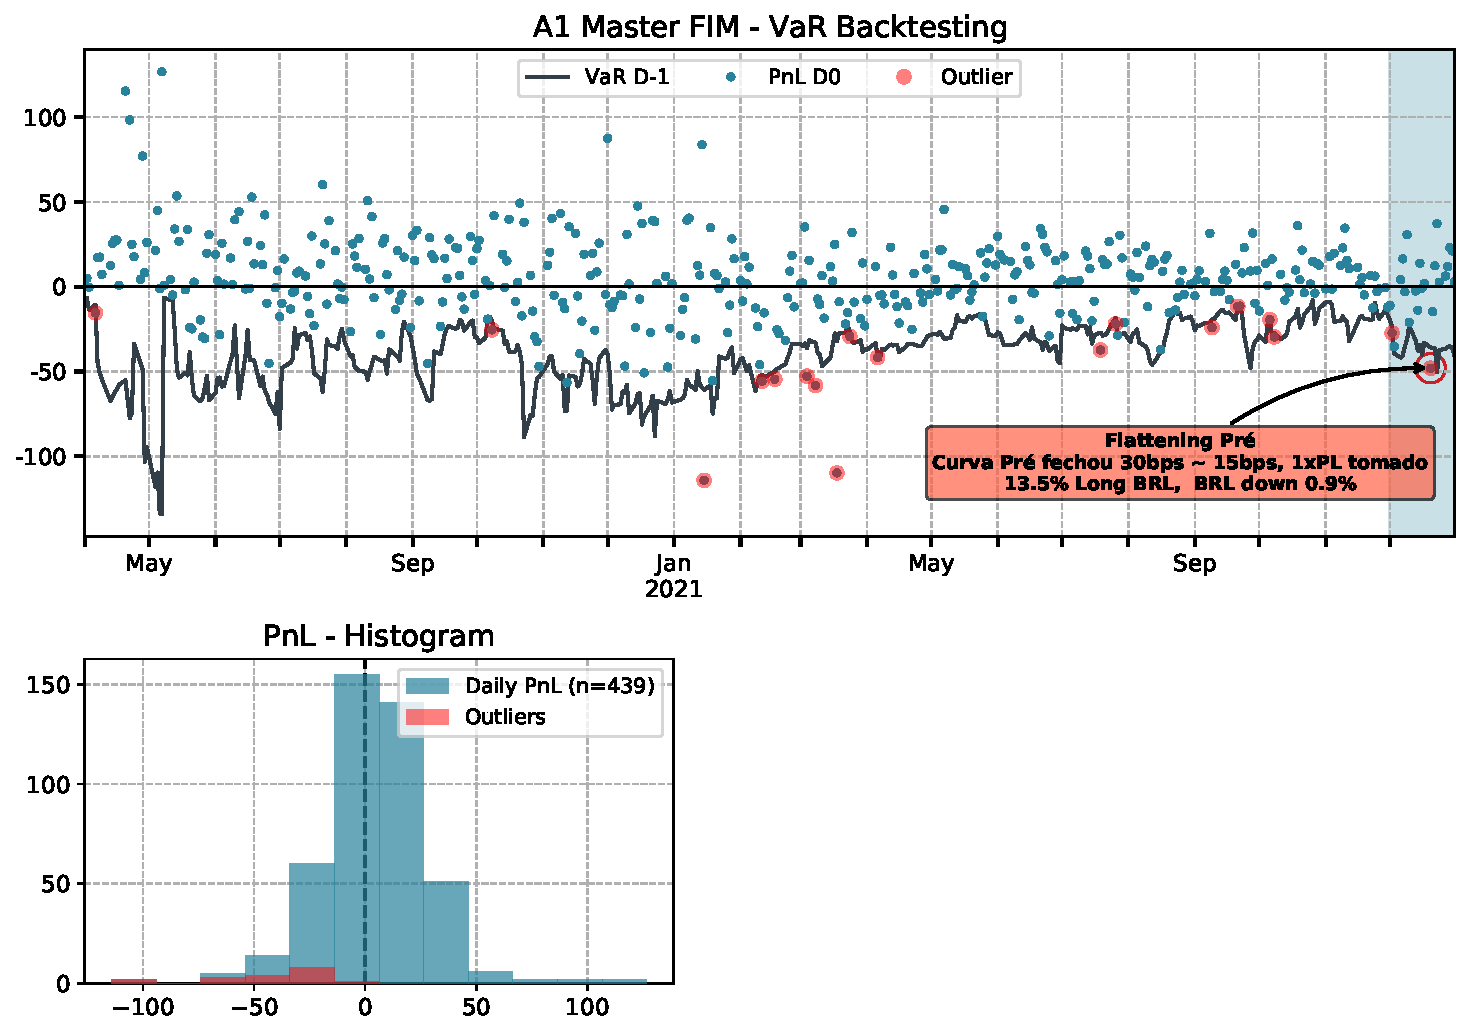
\includegraphics[width=0.90\linewidth]{figuras/20211231_A1 Master FIM_backtest_2021-12-20.pdf}
		}
		\only<4>{
			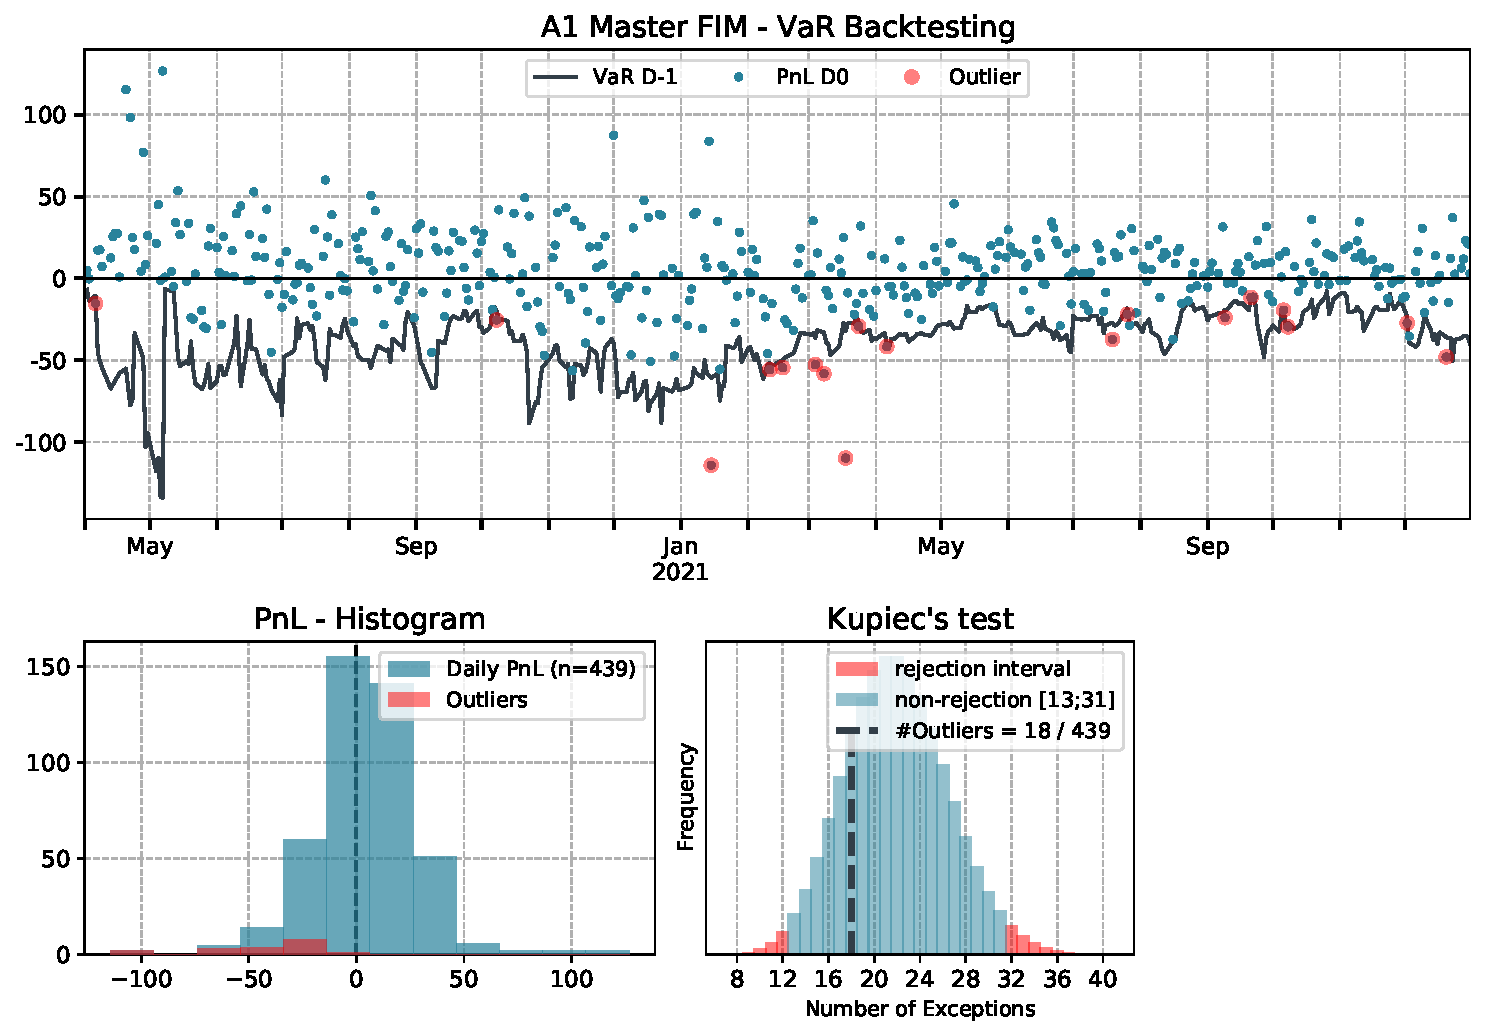
\includegraphics[width=0.90\linewidth]{figuras/20211231_A1 Master FIM_backtest_2.pdf}
		}
		\only<5>{
			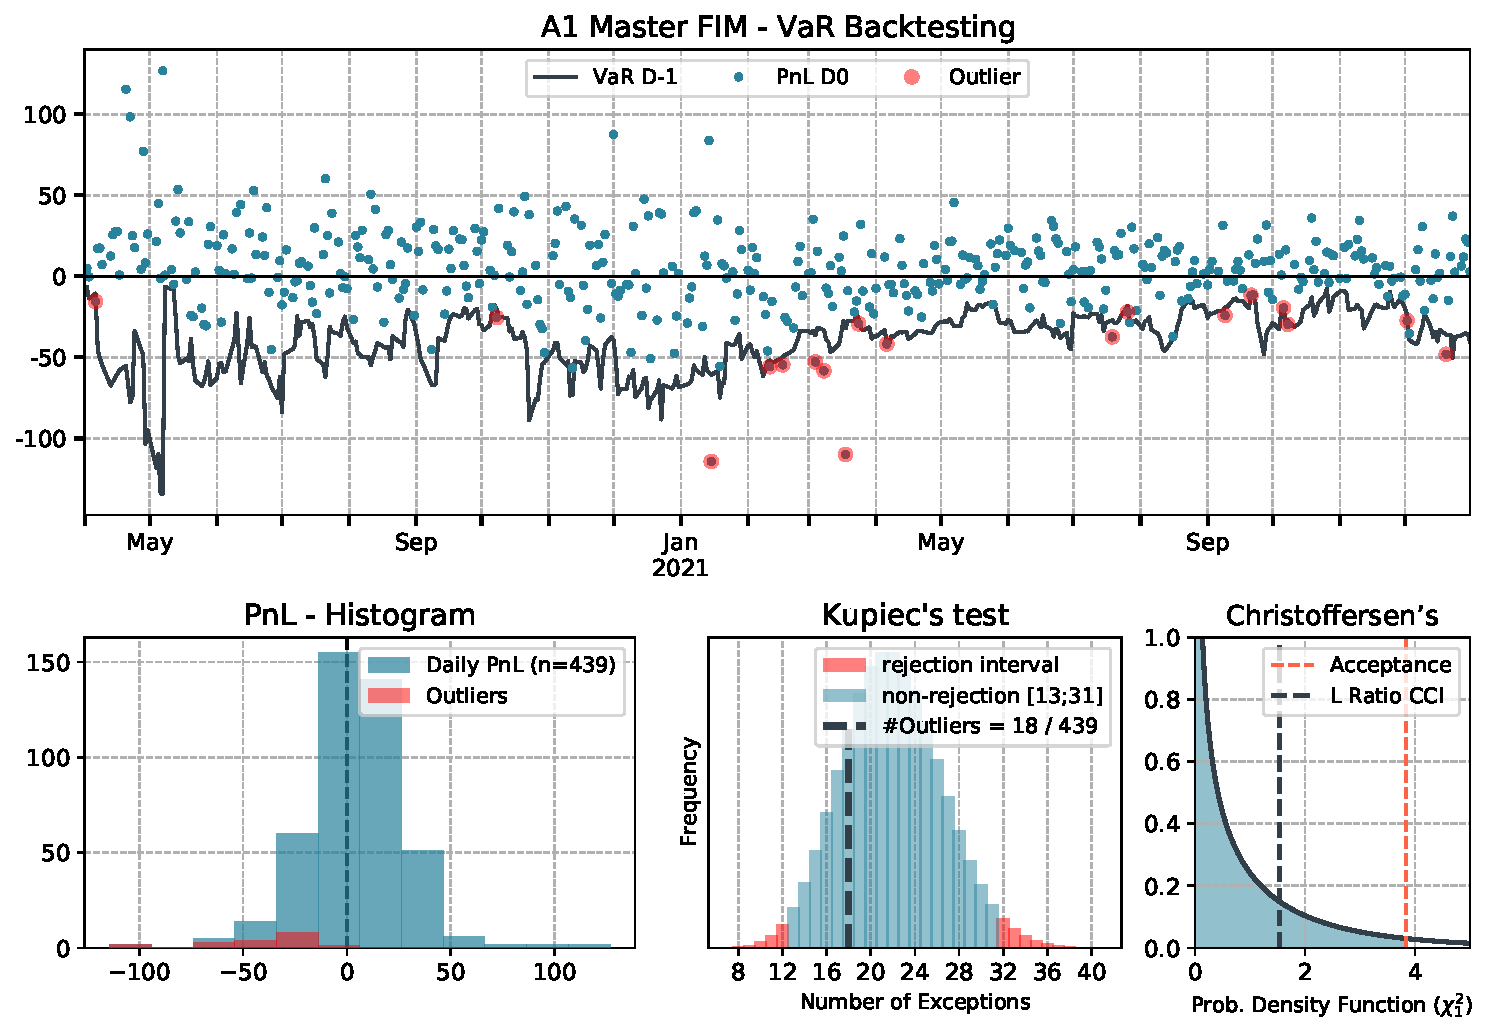
\includegraphics[width=0.90\linewidth]{figuras/20211231_A1 Master FIM_backtest_3.pdf}
		}

	\end{columns}
\end{overlayarea}
\end{frame}

\begin{frame}{Composição de Risco}
		\centering
	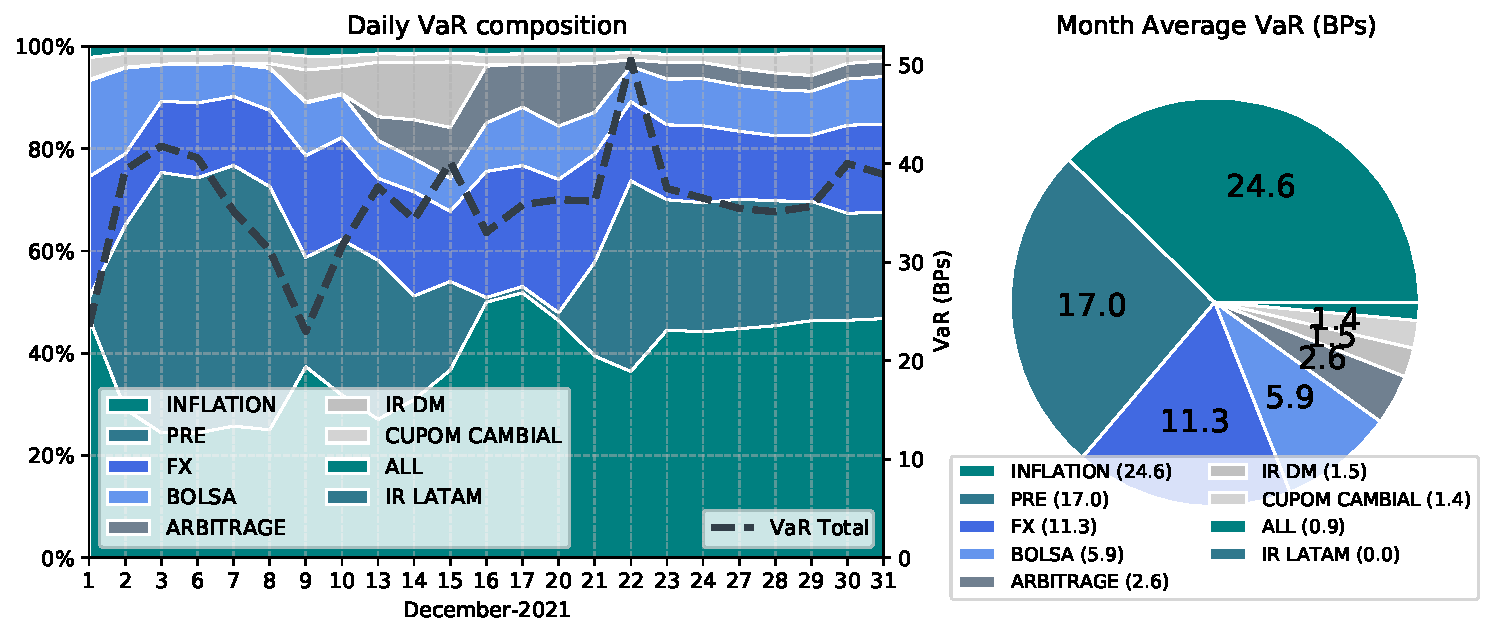
\includegraphics[width=0.99\textwidth]{figuras/20211231_hist_var.pdf} %month_var.py
\end{frame}

%%%%%%%%%%%%%%%%%%%%%%%%%%%%%%%%%%%%%%%%%%%%%%%%%%%%%%%%%%%%%
\section[Limites]{Acompanhamento de Limites}
\begin{frame}{Violações de Limites e Alertas}
	\centering
	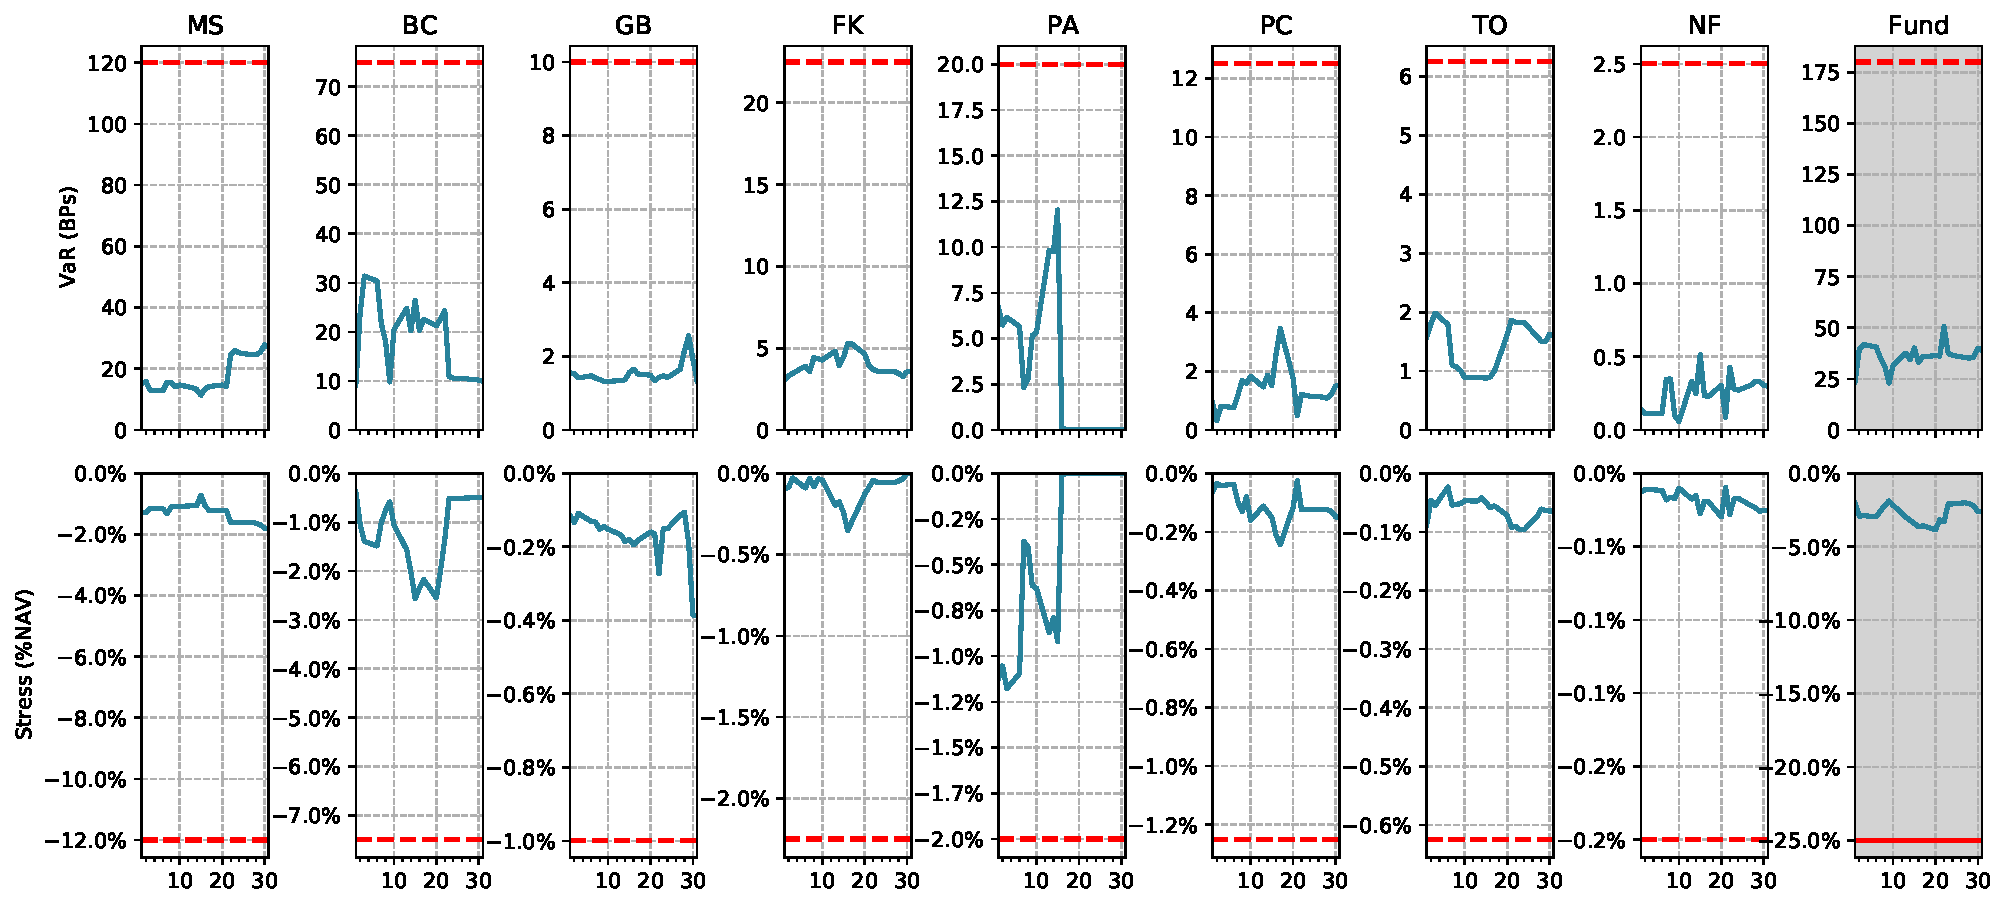
\includegraphics[width=0.99\textwidth]{figuras/211201_211231_trader_var_stress.pdf}%limits.py
\end{frame}

\begin{frame}{Rolagem do mês anterior}
	\centering
	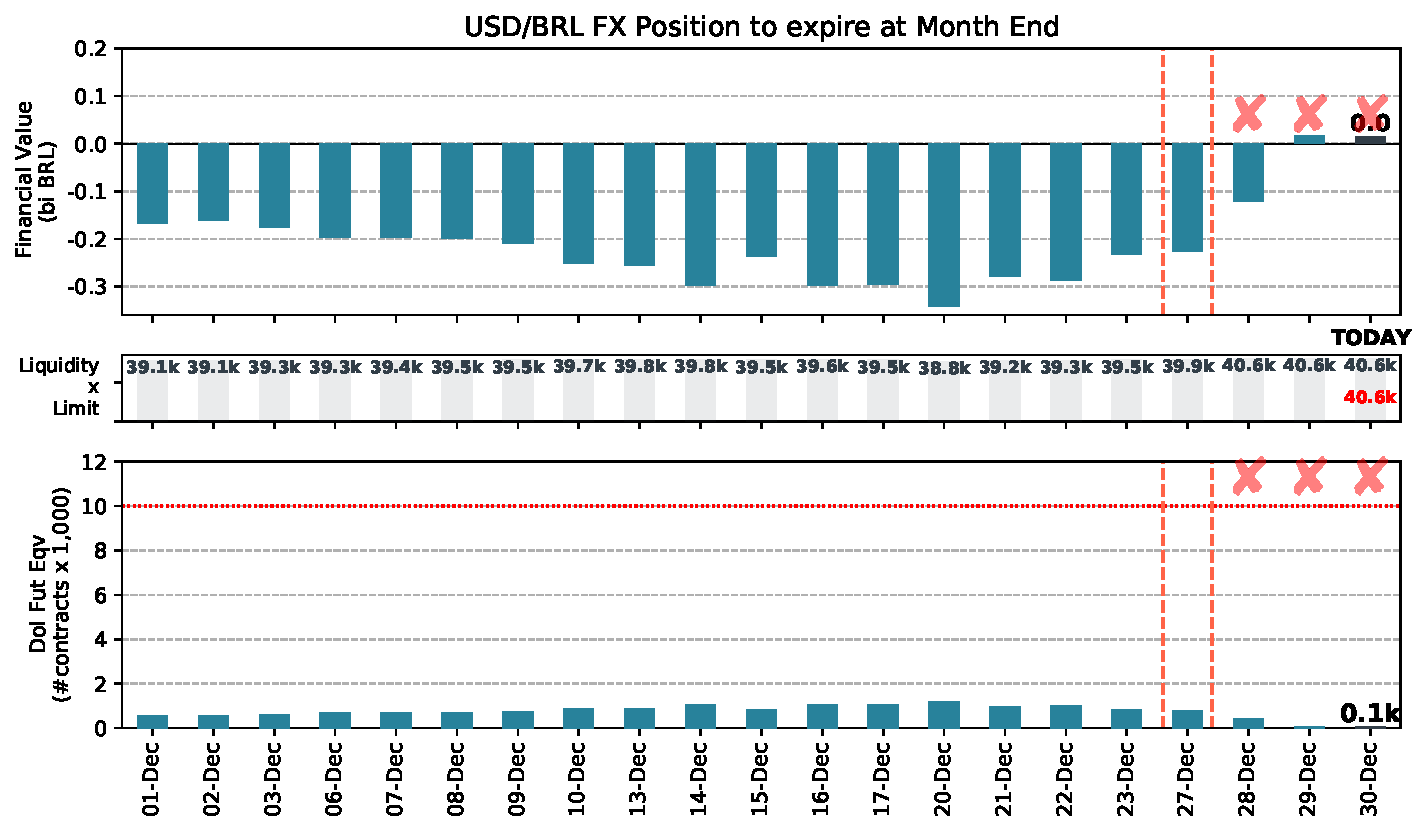
\includegraphics[width=0.77\textwidth]{figuras/20211230_A1 Master FIM_rolagem.pdf}  
\end{frame}

%%%%%%%%%%%%%%%%%%%%%%%%%%%%%%%%%%%%%%%%%%%%%%%%%%%%%%%%%%%%%
\begin{frame}{Política de Gestão de Risco de Liquidez - ANBIMA}
	\begin{itemize}
		\item {\color{blue1} Formulação da Política:}\\
		\small{Redação baseada na Política Interna de Risco e exigências da ANBIMA.}\\
		\item {\color{blue1} Implementação de Controles:}\\
		\small{Desenvolvimento dos processos complementares descritos na política.}\\
		\centering
		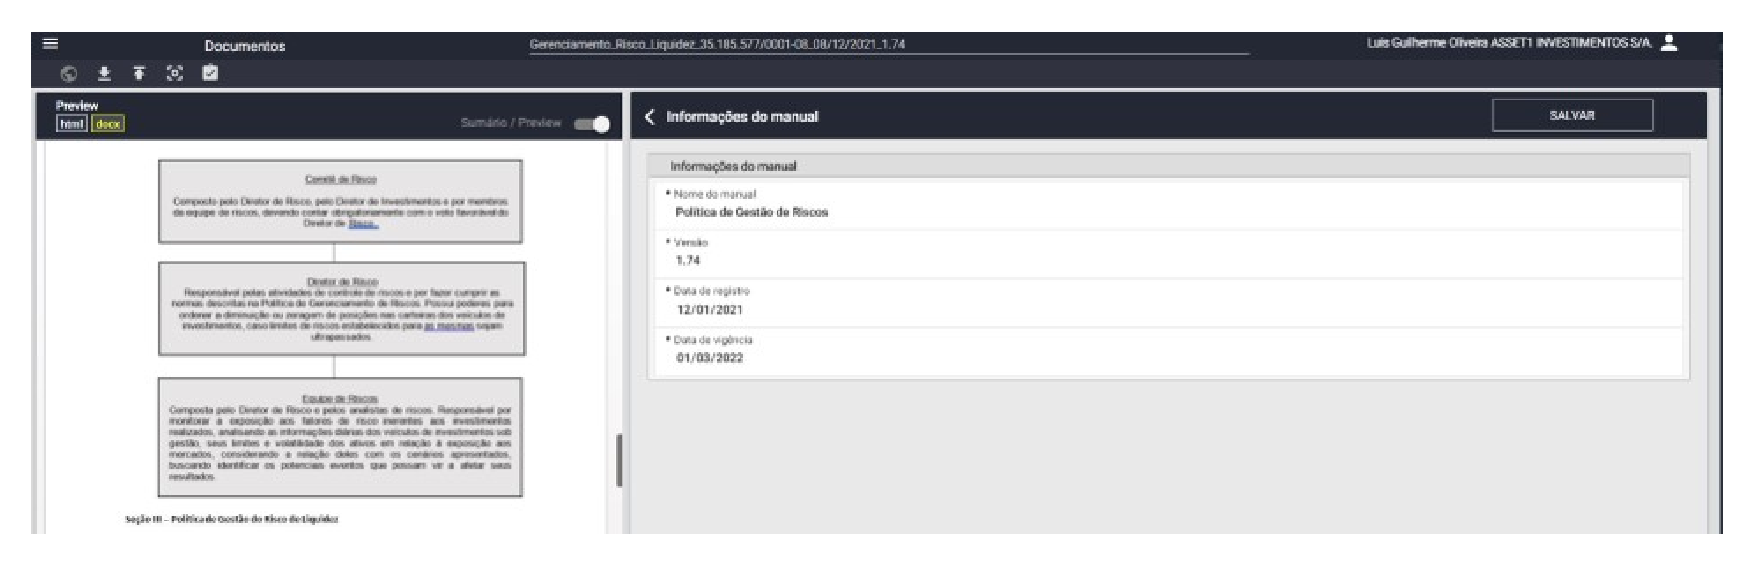
\includegraphics[width=0.77\textwidth]{figuras/Looplex - PRV.pdf}
	\end{itemize}
\end{frame}

%%%%%%%%%%%%%%%%%%%%%%%%%%%%%%%%%%%%%%%%%%%%%%%%%%%%%%%%%%%%%
\section[Risco]{Controles de Risco e Relatórios}
\begin{frame}{Permissionamento do Banco de Dados}
	Solução a ser implementada inclui configurações de infra-estrutura e retrabalho nos scripts implementados pelo consultor anterior.\\
	Próximos passos:
	\begin{itemize}
		\item {\color{blue1} Configuração dos Grupos do Azure Active Directory:}\\
		\large{Setup de grupos de usuários e permissões.}\\
		\item {\color{blue1} Teste das Permissões de Usuário:}\\
		\large{Retomar procedimentos de teste com os quatro usuários já estabelecidos.}\\
		\item {\color{blue1} Implementar Conexão via Script Python:}\\
		\large{Implementar módulo de conexão com o Banco de Dados que será utilizado por \emph{todos} os scripts.}\\
	\end{itemize}
\end{frame}

\end{document}